
\begin{figure}
	\centering
	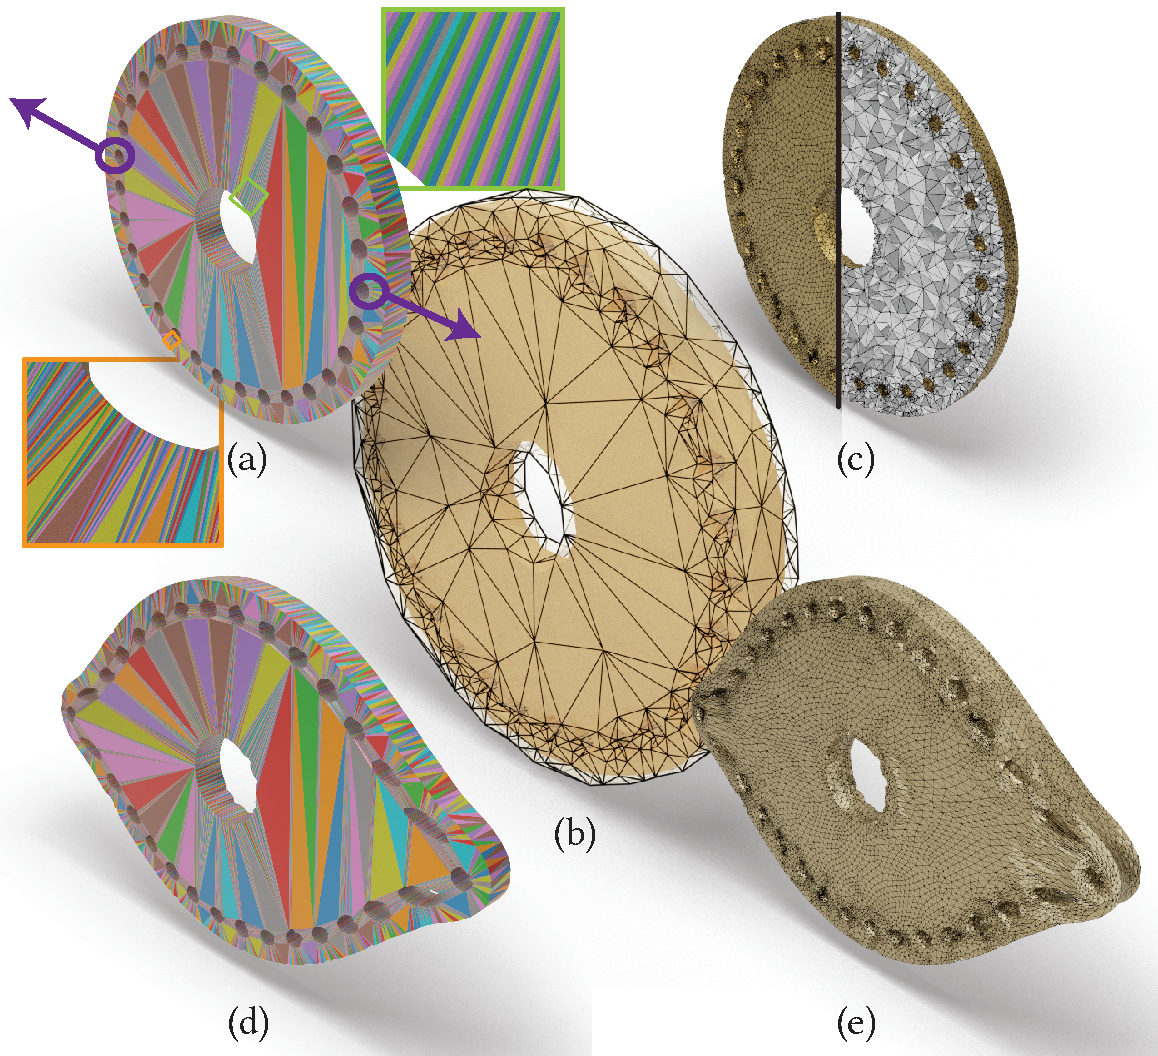
\includegraphics[width=\linewidth,draft=false]{prism-tex/figs/teaser_edit.pdf}
    \caption{A low-quality mesh with boundary conditions (a)
    is remeshed using our shell (b)
    to maintain a bijection between the input and the remeshed output.
    The boundary conditions (arrows in (a)) are then transferred to the high-quality surface (c),
    and a non-linear elastic deformation is computed %with PolyFEM%TODO
    on a volumetric mesh created with TetGen (\revision{e}).
    The solution is finally transferred back to the original geometry (\revision{d}).
    Note that in this application setting both surface and volumetric meshing \revision{can be hidden from} the user, \revision{who} directly specifies boundary conditions and analyses the result on the input geometry.}
    
    % \vspace{-1em}
    \label{prism:fig:teaser}
\end{figure}

\section{Introduction}
\label{sec:introduction}

Triangular meshes are the most popular representation for discrete surfaces, due to their flexibility, efficiency, and direct support in rasterization hardware. Different applications demand different meshes, ranging from extremely coarse for collision proxies, to high-resolution and high-quality for accurate physical simulation.
%
For this reason, the adaptation of a triangle mesh to a specific set of criteria (surface remeshing) is a core building block in geometry processing, graphics, physical simulation, and scientific computing.

In most applications, the triangular mesh is equipped with attributes, such as textures, displacements, physical properties, and boundary conditions (Figure~\ref{prism:fig:teaser}). Whenever remeshing is needed, these properties must be transferred on the new mesh, a task which has been extensively studied in the literature and for which robust and generic solutions are still lacking (Section \ref{sec:related}). 
Defining a \revision{continuous} bijective map, \revision{more precisely, a homeomorphism where the inverse is also continuous,} between two \revision{geometrically close}  piecewise-linear meshes of the same topology is a difficult problem, even in its basic form, when one of these meshes is obtained by adapting the other in some way (e.g., coarsening, refining, or improving triangle shape).a
Common approaches to this problem are Euclidean projection
\cite{jiao2004overlaying}, parametrization on a common domain \cite{praun2001consistent,kraevoy2004cross,lee1998maps}, functional maps \cite{Ovsjanikov:2012}, and generalized barycentric coordinates \cite{Hormann:2017:GBC}.  However, the problem is not fully solved, as all existing methods, as we discuss in greater detail in Section~\ref{sec:related},
 often fail to achieve bijectivity and/or sufficient quality of the resulting maps when applied to complex geometries. %geometrical models.
\revision{Our focus is on correspondences between meshes obtained during a remeshing procedure, instead of solving the more general problem of processing arbitrary mesh pairs.}

In this work, we propose a general construction designed to enable attribute mapping between geometrically close (in a well-defined sense) meshes by jointly constructing: (1) a shell $\S$ around triangle mesh $\T$ spanned by a set of prisms, inducing a volumetric vector field $\V$ in its interior and (2) a projection operator $\P$ that bijectively maps surfaces inside the shell to $\T$, as long as the dot product of the surface face normals and $\V$ is positive
(we call such a surface a \emph{section} of $\S$).
Given a surface mesh $\T$ and its shell $\S$, it is now possible to exploit the bijection induced by $\P$ in many existing remeshing algorithms by adding to them an additional constraint ensuring that the generated surface is a section of a given shell.

As long as the generated mesh is a section, the projection operator $\P$ can be used to transfer application-specific attributes. At a higher level, the middle surface of our shell can be seen as a common parametrization domain shared by sections within the shell: differently from other methods that map the triangle meshes to a disk, region of a plane, a canonical polyhedron, or orbifolds, our construction uses an explicit triangle mesh embedded in ambient space as the common parametrization domain.
This provides additional flexibility since it is adaptive to the density of the mesh and naturally handles models with high genus, while being numerically stable under floating-point representation (and exact if evaluated with rational arithmetic). The downside is that it is defined only for sections contained within the shell. \revision{
    The construction and optimization of our shell, and corresponding bijective mapping, is computationally more expensive than remeshing-only methods: our algorithms takes seconds to minutes on small and medium sized models, and might take hours on the large models in our tests.}

We evaluate the robustness of \revision{the proposed}approach by constructing shells for a subset of the models in Thingi10k \cite{zhou2016thingi10k} and in ABC \cite{Koch_2019_CVPR} (Section \ref{sec:results}). We also integrate it in six common geometry processing algorithms to demonstrate its practical applicability (Section \ref{sec:applications}):
\begin{enumerate}
    \item \emph{Proxy}.
    The creation of a proxy, high-quality remeshed surface to solve PDEs (e.g., to compute geodesic distances or deformations), avoiding the numerical problems caused by a low-quality input in commonly used codes.
%    without requiring any change in existing codes,
    Bijective projection operators associated with a shell enable us to transfer boundary conditions to the proxy mesh, compute the solution on the proxy, and then transfer the solution back to the original geometry.
    \item \emph{Boolean operations.} The remeshing of intermediate results of Boolean operations, to ensure high-quality intermediate meshes while preserving a bijection to transfer properties between them.
    \item \emph{Displacement Mapping.} The automatic conversion of a dense mesh into a coarse approximation and a regularly sampled displacement height map. Our method generates a  bijection that allows us to bake the geometric details in a displacement map.
    \item \emph{Tetrahedral Meshing.} The conversion of a surface mesh of low quality into a high-quality tetrahedral mesh, with bijective correspondence.
    \item \emph{Geometric Textures.} Generation of complex topological structures using volumetric textures mapped to the volumetric parametrization of a simplified shell defined by $\P$. Our analysis on the initial shell also complements the literature on shell maps.
    \item \emph{Nested Cages.} A robust approach to generate a coarse approximation of a surface for collision checking, cage-based deformation, or multigrid approaches.
\end{enumerate}

Our contributions are:
\begin{enumerate}
    \item An algorithm to build a prismatic shell and the corresponding projection operator around an orientable, manifold, self-intersection free triangle mesh with arbitrary quality;
    \item A new definition of bijective maps between \revision{\emph{close-by} discrete} surfaces;%, closed under rational representation and at the same time efficient and robust to evaluate in floating-point;\ZJ{Not shown}
    \item A reusable, reference implementation \revision{provided at \url{https://github.com/jiangzhongshi/bijective-projection-shell}}.
\end{enumerate}
